\documentclass[conference]{IEEEtran}
\usepackage{fullpage}
\usepackage{amsmath}
\usepackage{cite}
\usepackage{url}
%\usepackage{authblk}
\usepackage{enumitem}
\usepackage{sidecap}
\usepackage{graphicx}
\usepackage{array}
\usepackage{wrapfig}
\usepackage[export]{adjustbox}
\graphicspath{ {images/} }

\usepackage[bottom]{footmisc}
%\usepackage[style=verbose-ibid, backend=bibtex]{biblatex}
%\usepackage[style=authoryear,autocite=footnote]{biblatex}
%\bibliographystyle{IEEEtran}
%\bibliography{refer}

\begin{document}
\title{Database Synchronization Model for Mobile Devices}

\author{\IEEEauthorblockN{Shreya Reddy\IEEEauthorrefmark{1}, \IEEEauthorrefmark{2}, Joao Domingos\IEEEauthorrefmark{3}, Mi-Young Choi\IEEEauthorrefmark{3} \IEEEauthorrefmark{4} B.Sri Ramya \IEEEauthorrefmark{5} V.Balakumar}
\IEEEauthorblockA{\IEEEauthorrefmark{1}Jack Baskin School of Engineering\\
University of California,Santa Cruz}
\IEEEauthorblockA{\IEEEauthorrefmark{2}School of Technology and Management\\
Polytechnic Institute of Leiria,Portugal}
\IEEEauthorblockA{\IEEEauthorrefmark{3}Dept. of Computer Science and Engineering\\ Korea University}
\IEEEauthorblockA{\IEEEauthorrefmark{4}School of Engineering\\
Sri Vasavi Engineering College,India}
\IEEEauthorblockA{\IEEEauthorrefmark{5}Dept. of Engineering and Technology \\
Raja College of Engineering and Technology,India}}

\date{}
\maketitle

\begin{abstract}

\footnote{Intended conference of submission: 2018 19th IEEE International Conference on Mobile Data Management (MDM) \url{https://ieeexplore.ieee.org/xpl/tocresult.jsp?isnumber=8411240/}}
\footnote{Choi, Mi-Young and Cho, Eun-Ae and Park, Dae-Ha and Bae, Jong-Youn and Moon, Chang-Joo and Baik, Doo-Kwon, ``A synchronization algorithm of mobile database for ubiquitous computing," In: 2009 Fifth International Joint Conference on INC, IMS and IDC, IEEE. 2009. pp.416--419.}
\footnote{Ramya, B Sri and Koduri, Shirin Bhanu and Seetha, M,``A stateful database synchronization approach for mobile devices," International Journal of Soft Computing and Engineering (IJSCE). 2012. pp.3.}In the recent times, high performance small mobile devices like smart mobile phone, PDA, Pocket PC have rapidly came into use and are recognized as a popular client device in ``ubiquitous environment". Since the existing synchronization solutions of mobile database are not independent from the database server the use of database dependent information like meta-data is used.

The paper talks about the Synchronization Algorithm based on Message Digest (SAMD) which is a database synchronization algorithm for Mobile Devices. This model is based on message digests to \footnote{J. Domingos and N. Simões and P. Pereira and C. Silva and L. Marcelino, ``Database synchronization model for mobile devices'', In: 2014 9th Iberian Conference on Information Systems and Technologies (CISTI), IEEE.2014. pp. 1--7.}synchronize relational databases between mobile devices and a server, in order to minimize the data transferred between the device and the server. SAMD resolves the problems mentioned above using only standard SQL queries. The paper also discusses about the SQL Anywhere, which is served as a high-performance server which illustrates\footnote{V. Balakumar. and I. Sakthidevi, ``An efficient database synchronization algorithm for mobile devices based on Secured Message Digest," In: 2012 International Conference on Computing, Electronics and Electrical Technologies (ICCEET). IEEE. 2012. pp.937-942.}  how various self-management features work in concert to provide a robust data management solution in zero-administration environments. 
\end{abstract}


\begin{IEEEkeywords}

Mobile Database; Synchronization; Message Digest; Ubiquitous; Relational Database; SAMD; SQL standard queries 
\end{IEEEkeywords}

%INTRODUCTION SECTION

\section{Introduction}
The recent advances in mobile technology have led to the emergence of a new computing environment and a variety of small sized devices such as smart mobile phones, PDAs, Pocket PCs have become so popular in the ubiquitous environment. The simple device that plainly receives calls and sends messages, has become a tool for storing a users personal data. Since mobile phones have a limited computing power it is highly dependent on batteries. Moreover, it channels information through narrow bandwiths, which makes continous access to the network difficult.

If the user tries to access a large-sized data, then the connection in the server side database becomes hard to maintain since it can be prone to disconnections. To achieve a stable data processing, mobile devices are embedded with databases. 

A mobile phone in a disconnected environment will result to an inconsistent data stored in the mobile database and the server side database. This is where synchronization techniques or algorithm comes into the picture that provides a solution for data inconsistency. Synchronization algorithms guarantees data integrity.

Developing mobile applications for mobile devices usually require a specific library that comes with the mobile database vendor. Otherwise, the developer has to modify the existing mobile application for a synchronization process to function correctly. This limitation greatly affects the flexibility, adaptability and extensibility of mobile systems.

This paper presents the design of a proposed synchronization model based on message digests (SAMD) as an aid to assit data synchronization between mobile database and the server-side database. The focus is to minimize the use of resources of mobile devices. SAMD resolves synchronization problems using only standard SQL queries. This does not produce timestamps and does not make use of stored procedures nor triggers. In conclusion, the SAMD is a effective solution for mobile database synchronization in ubiquitous environment. Since the SAMD techniques are not specific to a particular database vendor, it can be used for any kind of combination of mobile database and server side database platforms.

%BACKGROUND SECTION

\section{Background Knowledge}
Synchronization technology can have an impact on the operation of mobile database. The lack of interdependent of the current synchronization solutions for mobile database and the database server since they utilize database dependent information like metadata or apply particular database functions like time stamp or trigger. Such functions give a weak position in ubiquitous environment due to the availability of various apps running on various servers. Due to this issue, synchronization algorithms based on Message Digest (SAMD) could improve the level of handling the issue. SAMD only uses standard SQL queries to solve the common synchronization problem. Moreover, it is possible to synchronize any data combination without considering the type of database's server. 

\begin{enumerate}[label=(\Alph*)]
\setlength\itemsep{1em}
\item  \textit{Synchronization}:

Synchronization that occurs between the client devices and remore servers happens through two mechanisms: upload and download. The upload process takes place first which corresponds to the transfer of data from client. On the other hand, download corresponds to the transfer of data from server to the client application.

The synchronization model in the Database Management System (DBMS) works with a number of clients connected to a server via network. There is usually a server and mobile devices that function as standard customers (shown in Fig.1). 

The whole framework consists of a server-side database, synchronization server(AnySyn) and multiple mobile devices with internal mobile databases. The server-side database keeps track of all the data thats required for business and the mobile database saves all the copies of data the user needs from the server-side. The server is located between the two databases to synchronize the date and maintain it. The AnySyn server performs synchronization based on the SAMD algorithm.

\begin{figure}[h]
	\centering
	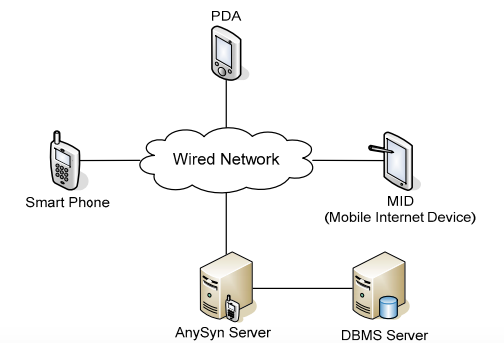
\includegraphics[width=1.1\linewidth]{sync.png} 
	\caption{Network Synchronization layout}
	\label{fig:sync1}
\end{figure}

\item \textit{Existing System}

This system uses synchronization algorithm based on comparison of message digest values of the selected rows of both server-side and mobile database thats needed for synchronization.

Database Management System provides several solutions for the synchronization of databases. But when using these solutions, mobile devices are highly dependent on a proprietary synchronization system. SQL Anywhere, for example, is a relational database management system (RDBMS) that uses few resources of the operting system which occupies low physical memory on the machine. A special synchronization technology, MobiLink, is used with SQL Anywhere system. This technology process consists of the client initiating a synchronization session by connecting to a remote database and compares all the modified rows from the previous session. It then uploads the compared rows to the server.The server then applies the changes to the required database and selects the rows that need to be sent to the client. The client receives the modifications and sends an acknowledgment back to the server.

\item \textit{Message Digest}

A message digest is a one-way hash function that maps a message with a random length hash value to a fixed length. The concept of message digest is defined by the formula, h = H(M), where h respresnts the message digest, H the hash function and M corresponds to the message of any length. Making a change in the message causes a change in the message digest value. Fig 2. represents how this message digest mechanism can be applied to a relational database to examine data identity between rows of two tables.

\begin{figure}[h]
	\centering
	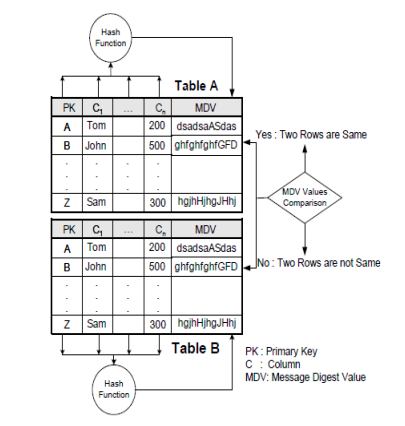
\includegraphics[trim={1cm 0 1.5cm 0},width=7.5cm]{data.png} 
	\caption{Message Digest in Data Tables}
	\label{fig:data1}
\end{figure}


Data in these two rows are identical if two rows in Tables A and B have the same message digest values. If the two values are different, it means that the two rows have one or more different column values. This mentod is useful in detecting inconsistency between two rows. When a row with inconsistency is detected, then the row is copied using the primary key in the direction of synchronization. This synchronization algorithm identifies a modified row without relying on the database's internal functions, logs or metadata to enable synchronization that is independent of the database vender. 

\item \textit{Rows Inconsistency}

Inconsistency refers to a state where the published data values in the database are different from the subscribed data in the mobile database. Table 1 displays every case for an inconsistency for a single row. The two databases add, delete and modify data independetly which makes inconsistency inevitable.

From Table 1, there are 16 cases. Cases 6,7.8 include the ADD function which cannot occur for a single row. For example, Case 7 the row added at the server side is different from the row modified at the client therefore it cannot be considered inconsistent.

\begin{table}[ht]
\centering
\setlength\tabcolsep{16pt}
\caption{Inconsistency Analysis}
\begin{tabular}{||c c c ||} 
	\hline
 C & Mobile DB & DB Server \\ [0.5ex] 
 \hline\hline
 1 & UC & UC \\ 
 	\hline
 2 & ADD & UC  \\
 	\hline
 3 & MOD & UC \\
 	\hline
 4 & DEL & UC  \\
 	\hline
 5 & UC & ADD \\
 	\hline
 6 & ADD & ADD  \\
 	\hline
 7 & MOD & ADD  \\
 	\hline
 8 & DEL & ADD  \\
 	\hline
 9 & UC & MOD  \\
 	\hline
 10 & ADD & MOD  \\
 	\hline
 11 & MOD & MOD  \\
 	\hline
 12 & DEL & MOD  \\
 	\hline
 13 & UC & DEL  \\
 	\hline
 14 & ADD & DEL  \\
 	\hline
 15 & MOD & DEL  \\
 	\hline
 16 & DEL & DEL  \\  
    \hline

\end{tabular}
\label{table:1}
\end{table}

\end{enumerate}

%SAMD ALGORITHM

\section{SAMD Synchronization Algorithm}
\begin{enumerate}[label=(\Alph*)]
\setlength\itemsep{1em}
\item  \textit{Objective of SAMD}

In order to guarantee independence of database and synchronization vender in ubiquitous environment, the SAMD algorithm must satisfy the following requirements.

 \begin{itemize}
	\item Independent of database

Does not use metadata or internal functions dedicated to a particular database.

	\item Synchronization using only standard SQL statements

Perform synchronization using only standard SQL queries and data manipulation language specified in ISO. Any data processing using trigger is not allowed.

	\item Disallows schematic modification of data table of the database server.

Synchronization must be performed independent from the existing data table schema. So, additional information such as time stamps cannot be added to the data table. 

	\item Disallows adding restrictions in implementing applications

There can be no restrictions such as performing additional works to an application code or having to use a specific library in order to perform synchronization. 
 \end{itemize}

\item  \textit{SAMD Synchronization Algorithm}

%EDIT THIS PART

The SAMD synchronization algorithm is applied for the table schema of the server-side database and the mobile database. Both databases have a data table (DSDT: Database Server Data Table, MCDT: Mobile Client Data Table) and a message digest table (DSMDT: Database Server Message
Digest Table, MCMDT: Mobile Client Message Digest Table). The data table contains the business data, and the message digest table stores the message digest value from the data table. The message digest table consists of a PK(primary Key) column of data table, message digest value (MDV) column, flag (F) column and mobile device ID (Mid) column. The flag column signals an inconsistency that has occurred in the corresponding column; therefore, the flag column is used
to identify a row that requires synchronization. The mobile device ID is a unique number of the mobile device, so this column is used to identify a mobile device that requires synchronization.

%EDIT THIS PART

In Fig. 3 , if a row's PK value is A1, this value is identical to the two message digest values and there is no need for synchronization. However, if a row has a PK value of C1, the value of MDV in MCMDT is different from the value of MDV in DSMDT and the MCMDT flag value is 1. Consequently, synchronization is necessary. The synchronization process is performed for each row to resolve all of the inconsistencies mentioned in Section II/B. For
example, if there is an inconsistency in row C1, synchronization takes place from the mobile database to the server-side database and DSDT's PK C1 row is replaced with the MCDT's C1 row.

\begin{figure}[h]
	\centering
	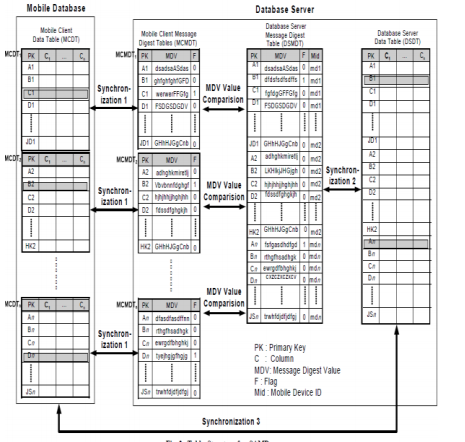
\includegraphics[trim={0.66cm 0.1cm 1.2cm 0.1cm},clip, width=0.9\linewidth, height=11cm]{explain.png} 
	\caption{Table Structure for SAMD}
	\label{fig:explain1}
\end{figure}



The synchronization algorithm consists of Synchronization 1, 2 and 3 as shown in Figure 2. Synchronization 1 and 2 synchronizes the data table and message digest table. Here, the message digest values are created with each row values of the data table, and the message digest values are compared with those of the message digest table. If the values are identical, there has been no change in the data and synchronization is not necessary. If the values 


\begin{figure*}
	\centering
	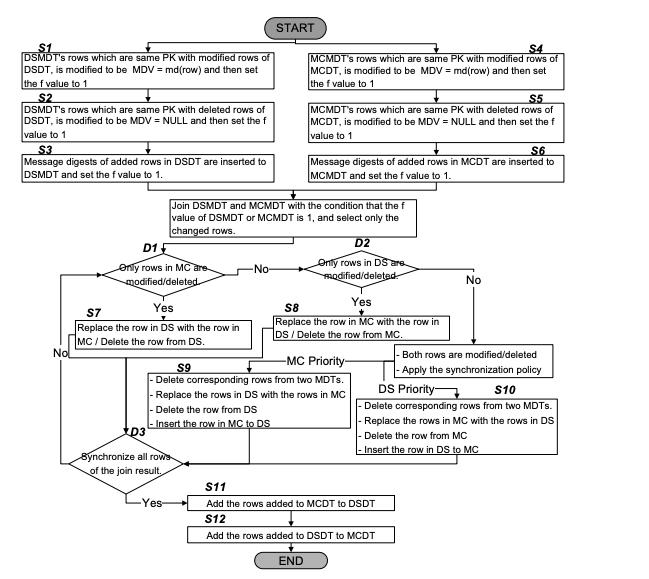
\includegraphics[width=\textwidth, height=12cm]{flowchart.png} 
	\caption{Flowchart for SAMD}
	\label{fig:flowchart1s}
\end{figure*}



are different, this means that the datatable value has been changed, in which case the message digest table has to be updated with new values and the flag has to be set to 1. The flag value is used to identify a row that needs synchronization. The database server has one DSMDT for every DSDT. Although the size of the MCMDT is smaller than that of the DSMDT, there is an MCMDT for every mobile device which has unique ID. When the mobile
device request synchronization, the mobile device ID value is sent database server side and then SAMD algorithms selects the rows from DSMDT whose value of Mid column is same to the mobile device ID value and Synchronization 2
is only applied with the selected rows. After SAMD algorithms analyze the type of inconsistency using the flag values of the two messages digest tables, Synchronization 3 is performed between two data tables for each inconsistent
type. Upon completion of synchronization, the flag of the synchronized row is set to 0 in the message digest table. Figure 3 exhibits the flow chart for the SAMD synchronization algorithm. Steps S1~S3 represent the
Synchronization 2 stage of Figure 2. When the DSDT and DSMDT are FullOuterJoined, DSDT rows for which StepsS1, S2 and S3 should be applied can be identified by using dangling rows. Steps S4~S6 indicate the Synchronization 1
stage. This stage involves synchronizing the MCDT and MCMDT, and the basic algorithm is identical to Steps S1~S3. However, the MCDT and MDMDT are internal data tables of different vendor databases that are physically
separated, so FullOuterJoin as in Steps S1~S3 is not feasible. In this case, a temporary table has to be created for the MCDT table to be copied to the server side, and Synchronization 1 process is performed, after which the copied data is deleted. This single transaction by batch processing guarantees independence of the SAMD algorithm for the database vender.  

Steps S7~S12 display the Synchronization 3 stage of Fig. 3. When the DSMDT and MCMDT are FullOuterJoined, the rows that are subject to synchronization and the inconsistent types are identified using the dangling rows and the DSMDT and MDCMDT flags and then the synchronization between the DSDT and MCDT is achieved.  Step S7 involves synchronizing a modified row or one deleted from the MCDT with the DSDT. Under the D1 condition, Step S7 searches for a row with an MCMDT flag value of 1 and a DSMDT flag value of 0. The flag values indicate that the row was modified or deleted from the MCDT. A null MDV column of the MDMDT signifies a deletion from the MCMT. Otherwise, there has been a modification. In the case of deletion, rows that correspond to the rows deleted from the MCDT should be deleted from DSDT, DSMDT and MDMDT. In the case of modification, the DSDT row value is
replaced with the MCDT row value, and DSMDT row value is replaced with the MDMDT row value. Upon completion of synchronization, the flag values of the synchronized rows of 



\end{enumerate}

%Proposed section 
\section{Proposed Solution}

In this section the proposed solution for synchronization model is presented. The main purpose of this model is to synchronize a mobile device database with a remote server's database, which is used to minimize the use of resources of the mobile devices.

The primary objectives that focus on minimizing the use of resources of the mobile devices are i) minimize the amount of data transmitted during the synchronization process ii) minimize the data processing of the mobile.

The secondary objectives are that synchronization model not be dependent on any proprietary implementation or any commercial application. And the database server not contain any information about the devices.

\begin{enumerate}[label=(\Alph*)]
\setlength\itemsep{1em}
\item  \textit{Network Architecture}

The architecture of this model is very similar to any architecture of the existing synchronization model, consisting of a server with a database and several client devices that synchronize the data with the server.
\begin{itemize}
 	\item[--] The client is the mobile device that essentially composed of a client application that makes data management business and a synchronization algorithm that makes the proposed algorithm of the synchronization client and a relational database management system that manages and manipulates the database to be synchronized with the server.

	\item[--] The server is mainly composed by a synchronization agent that implements the proposed algorithm of the  server. This agent also provides remote methods for synchronization.
\end{itemize}

\item  \textit{Table Structure : Client}

In order for the data to be properly synchronized with the server, the client must have the following table structure mentioned below.
\begin{itemize}
	\item \textit{ Private Key}

The unique identifer of a record. It's only valid in the client's database.

	\item  \textit{ Public Key}

The primary key used by the server. Its used to do mapping between the records in the database of a particular client and the records in the database of the server.

	\item  \textit{Business Data}

The content of the record that synchronizes the matter. The information is managed by the client application.

	\item \textit{Modification offline state}

Its the current state of the record and it also informs on any offline changes that are made.

	\item \textit{Actual Message Digest Client}

Its the message digest produced by the hash function in which the input of the function are business data present in the current version of the record in the database of the client.

	\item \textit{Last Sync Message Digest}

A message digest produced by the hash function in which the input of the function are business data present in the latest version of the record in the database of the server.

	\item \textit{Consistent}

When the synchronization process takes place, it makes sure whether the record is consistent with the one presented.
\end{itemize}
	 

\item  \textit{Table Structure : Server}
\begin{itemize}
	\item \textit{Primary Key}

Its the unique identifier of the table.

	\item \textit{Business Data}

The content of the record that synchronizes the matter. The information is managed by the client application.

	\item \textit{Actual Message Digest}

Its the message digest produced by the hash function, in which the input function is the business data present in the current version of the database server. This gets updated whenever the business data is modified.


	\item \textit{Active}

Tells whether the record is active or not. A record is never removed from the database server, its just disabled.
\end{itemize}

\item  \textit{Offline Mode}

Most of the times, mobile devices do not have any connection to the network, hence the remote servers are used. So, mobile devices must be prepared to work in offline mode i.e. without a connection to the server. In the synchronization model, the client application is always assumed to be offline. It is also necessary to preserve the manipulation made in the database by the client application. By doing this during the synchronization process it knows which records need to be synchronized from the client to the server.

\item  \textit{Synchronization Algorithm : General}

This algorithm consists of two phases: Sync Out and Sync In. The sync out occurs first where the synchronization of the client to the server is made. And then the sync in takes place.

\item  \textit{Synchronization Algorithm : Client}

The sync out process takes place in the client. A diagram of how the process takes place is shown below.

\begin{figure}[h]
	\centering
	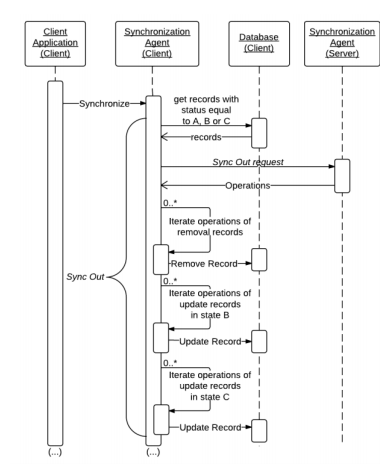
\includegraphics[trim={1cm 0.3cm 0.9cm 1cm},clip, width=7cm, height = 9cm]{sync-out.png} 
	\caption{Sequence in the Phase of Sync Out (Client)} 
	\label{fig:sync-out1} 
\end{figure}

After the sync out request, the server returns a set of operations that are performed in the database client. The operations include: removal record, update record in state B and update record in state C.


\begin{table}[h!]
\centering
\caption{Types of operations returned by the server}
\setlength\tabcolsep{8pt}
\begin{tabular}{ | m{5em} | m{15em}| } 
\hline
\textbf{Type of Operation} & \textbf{Attributes returned by the server} \\
\hline
Removal record& Confirmation flag of the deactivation record; Public key \\ 
\hline
Update record in the state B  & Confirmation flag of the insertion record;
Primary key of the record in the database client;
Primary key of the record in the database server  \\ 
\hline \
Update record in the state C  & Confirmation flag of the update record;
Primary key of the record in the database server  \\ 
\hline 
\end{tabular}
\label{table:2}
\end{table}

After receiving the response from the server, the client handles the database in accordance with the operations returned by the server.

\begin{table}[h!]
\centering
\caption{MANIPULATIONS IN THE \\ DATABASE CLIENT (SYNC OUT) }
\setlength\tabcolsep{8pt}
\begin{tabular}{ | m{5em} | m{15em}| } 
\hline
\textbf{Type of Operation} & \textbf{Manipulations in the database client } \\
\hline
Removal record& Remove record. \\ 
\hline
Update record in the state B  & Update the public key attribute with the primary
key received;
Update the status attribute of offline operations
with the D value;
Update the Last Sync Message Digest attribute
with the attribute value Actual Message Digest;
Consistent update the attribute with the value Y.  \\ 
\hline
Update record in the state C  & Update the status attribute of offline operations
with the D value;
Update the Last Sync Message Digest attribute
with the attribute value Actual Message Digest;
Consistent update the attribute with the value Y.   \\ 
\hline 
\end{tabular}
\label{table:3}
\end{table}

The sync in process verifies the generic process on the client's side. This is shown in Fig 5. 

\begin{figure}[h]
	\centering
	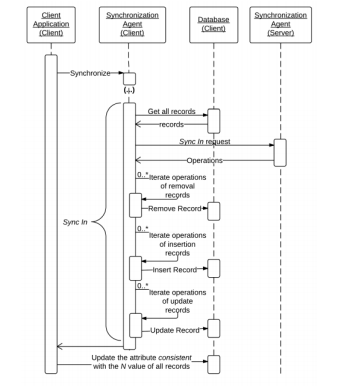
\includegraphics[trim={1cm 0 1cm 0},clip, width=8.5cm]{sync-in.png} 
	\caption{Sequence Diagram in the Sync In phase (Client)}
	\label{fig:sync-in1}
\end{figure}


 During the sync in phase, a request is made to ther server wherer all the records that are present in the client database are sent to the server. The server returns a set of operations that are to be performed on the database client, which contains the following types of operations: insert, update and delete. This is shown in TABLE IV.

\begin{table}[h!]
\centering
\caption{TYPE OF OPERATIONS\\ RETURNED BY THE SERVER (SYNC IN)}
%\setlength\tabcolsep{20pt}
\begin{tabular}{ | m{5em} | m{10em}| } 
\hline
\textbf{Type of Operation} & \textbf{Attributes returned by the server} \\
\hline
Removal record& Public key \\ 
\hline
Insertion record & Public key; Business data; Actual Message Digest.   \\ 
\hline
Update record & Public key; Business data; Actual Message Digest.   \\ 
\hline 
\end{tabular}
\label{table:4}
\end{table}

After a call is made to the server, the client handles the database in accordance with the operations returned by the server.

\begin{table}[h!]
\centering
\caption{HANDLING IN DATABASE CLIENT (SYNC IN)}
\begin{tabular}{ | m{5em} | m{15em}| } 
\hline
\textbf{Type of Operation} & \textbf{Manipulations in the database client} \\
\hline
Removal record& Remove record. \\ 
\hline
Insertion record & Insert record (Public Key, Business data and Actual
Message Digest);
Update the attribute of state operations offline with the
D value;
Update the Last Sync Message Digest attribute with
the attribute value Actual Message Digest.  \\ 
\hline
Update record & Update record (Business data and Actual Message
Digest);
Update the status attribute of offline operations with
the D value;
Update the Last Sync Message Digest attribute with
the attribute value Actual Message Digest.  \\ 
\hline 
\end{tabular}
\label{table:5}
\end{table}

\item  \textit{Synchronization Algorithm : Server}

\begin{figure}[h]
	\centering
	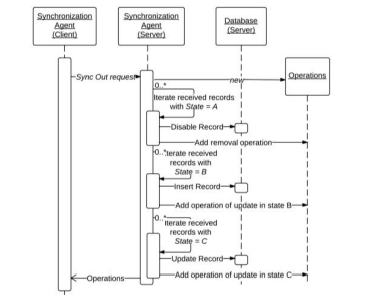
\includegraphics[trim={1.3cm 0.4cm 1.5cm 0.4cm},clip, width=1.1\linewidth]{SERVER.png} 
	\caption{Sequence during the Sync Out phase (Server)}
	\label{SERVER1}
\end{figure}

In the sync out process the request made to the server have states A,B or C and these can be received. Each of these states are iterated. Every manipulation thats successfully done by the server is recorded and sent back to the client.

\end{enumerate}

%MODEL ANALYSIS SECTION
\section{Model Analysis}
First, an analysis is made for the amount of data transferred. Regarding the Sync Out phase, there was an effort to reduce the amount of data that is sent at this stage; it is only sent to the server records that somehow were changed by the client application and, regarding the attributes of those records, the only records that are sent are the ones indispensable for a correct synchronization. During the Sync In phase, all the records in the device are sent to the server but only containing the essential attributes. It becomes very useful to send the information of all the records because, in doing so, the server has an overview of the data present in the device and thus can accurately calculate the required operations so that the database client becomes consistent with the database server. The great advantage of the server knowing exactly what the necessary operations are is not to transmit data that
could be discarded by the device. 

\begin{figure}[h]
	\centering
	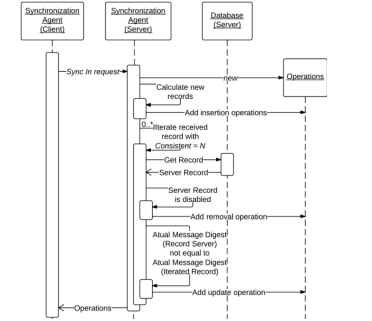
\includegraphics[trim={1cm 0.3cm 1.2cm 0.2cm},clip, width=1.1\linewidth]{ser.png} 
	\caption{Sequence Diagram of Sync In phase (Server)}
	\label{ser1}
\end{figure}

The processing done by the mobile device during each synchronization phase is very simple, and it always consists of the following three general steps: reading records from the
database, calling the sending server logs and, finally, applying the operations on the data returned by server. During the Sync Out phase, the device never has to do complex calculations of the records needed or not needed to be sent to the server because there is a notation of which records need to be sent. Both in Sync In and Sync Out phases, the content returned
represents the database operations, and so there is a direct mapping between these operations and the manipulations in the database. This prevents the device of having to do complex
calculations of which records need or need not to be synchronized. To highlight the difference, consider the following example: if the device received all the server logs, the device needed to process which records should be inserted, removed and modified. In our model, this processing is done on the server, thus minimizing the processing performed by the device. 

%IMPLEMENTATION AND EVALUTION SECTION
\section{Implementation and Evaluation-Results}

\begin{enumerate}[label=(\Alph*)]
\setlength\itemsep{1em}

\item  \textit{Performance Evaluation}

The SAMD algorithm was implemented using Java and it was linked with databases using JDBC(Java Database Connectivity). The business synchronization solution, which is vender-independent of server-side database and has a middle-tier architecture, was used to compare SAMD. The hash function MD5 was used to produce the message digest. The synchronization agent(server) was implemented using the PHP script.

For performance evaluation, the commerical RDBMS and mobile database were installed on one machine to eliminate the network effect factors.First, 500 randomly generated rows were inserted into RDBMS, sent through synchronization and the same 500 rows were inserted into mobile database. Then, 50 rows were inserted into RDBMS, 

\begin{figure}[h]
	\centering
	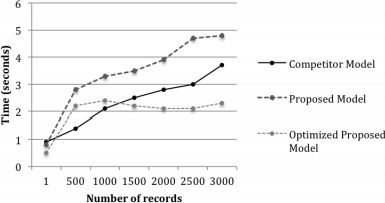
\includegraphics[width=1.1\linewidth]{newgraph.png} 
	\caption{Time Spent in Synchronization Client to Server (in seconds)}
	\label{graphs1}
\end{figure}

\begin{figure}[h]
	\centering
	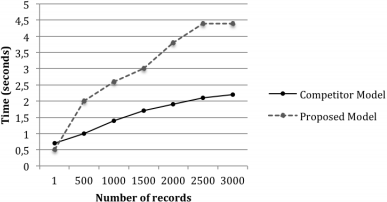
\includegraphics[width=1.1\linewidth]{graph.png} 
	\caption{Time Spent in Synchronization Server to Client (in seconds) }
	\label{graphss1}
\end{figure}

and then inserted another 50 rows into mobile database. Afterwards, 50 rows were deleted from mobile database and another 50 rows modified. The modified and deleted data were programmed to be equally spaced among the 500 rows. In this condition, performance was evaluated by comparing the synchronization time of SAMD and the commercial synchronization solution. Results shown in the graph (Fig 9 and 10). 

The synchronization time was evaluated ten times using different data in the same conditions and the average was calculated. This is shown in the table below.


\begin{table}[h!]
\centering
\caption{PERFORMANCE RESULTS }
\setlength\tabcolsep{8pt}
\begin{tabular}{||c c c ||} 
 \hline
 \textbf{SAMD} & \textbf{Commercial} & \textbf{Difference}\\ 
 \hline 
 1.55 & 2.18 & 0.64 \\
 \hline
\end{tabular} 
\label{table:6}
\end{table}



The table represents the performance evalution result that SAMD is faster than the commercial synchronization solution by an average of 0.64 seconds.

For the commercial synchronization solution,a synchronization SQL was used. Furthermore, some cases in TABLE VI are not supported.
Therefore, the evaluation could not be performed for all cases listed in TABLE VI but only for the four cases mentioned above. The commercial synchronization solution requires that additional data table, procedures and triggers be created for synchronizing with a server-side database that is not a same vender of the commercial synchronization solution. The vender of the commercial synchronization solution and the mobile database must be the same, but SAMD mandates no restrictions regarding the types of the server-side databases.

\item  \textit{Quality Evaluation}

A SAMD algorithm was designed to maintain the objective of algorithm as mentioned aboveThe
mentioned objectives are problems that existing commercial synchronization products have, so if these objectives are not achieved, the wide use property for application of synchronization algorithm would not be fulfilled. The widely used technologies for mobile database synchronization are timestamp and snapshot technique, using staging table in middletier,
integrated RDBMS which use message and before-image technique. The commercial synchronization solutions which use these technologies were compared with SAMD on the basis of mentioned algorithm objectives. Table VII

\begin{table}[h!]
\centering
\caption{QUALITY EVALUATION }
\setlength\tabcolsep{2.5pt}
\begin{tabular}{|m{5em}| m{5em}| m{5em}| m{5em}| m{5em}|} 
 \hline
\textbf{Objective} & \textbf{Timestamp and Snapshot} & \textbf{Staging
Table[5]} & \textbf{Integrated DBMS } & \textbf{SAMD}  \\ 
 \hline\hline
 \textbf{O1}&O&X&X&O\\ 
 \textbf{O2}&X&X&X&O\\
 \textbf{O3}&O&O&O&O\\
 \textbf{O4}&O&O&O&O\\ 
 \hline 
\end{tabular}
\label{table:7}
\end{table}

represents algorithm designing objectives and maintaining or not as to objectives of each technologies/SAMD. 

\end{enumerate}

%\section{Future Work}
%Looking at the growing number of businesses that are expanding to mobile environments, synchronization models like the one proposed above is very important. So, in the future, the focus will continue to be in the reduction of resources used by mobile devices.

%COnclusion section 
\section{Conclusion}
The paper has suggested an SMAD synchronization
algorithm based on message digest for synchronizing between
server-side databases and mobile databases. The SAMD
algorithm is performed with only SQL functions of relational
databases, so that it is not dedicated to particular venders and
is available for use in combination with any server-side
databases and mobile databases. Therefore, extensibility,
adaptability and flexibility are guaranteed when a mobile
business system is authorized. This feature is important in
order to build efficient mobile business systems because the
upcoming mobile business environment has heterogeneous
characteristics in which diverse mobile devices, mobile
databases and RDBMS exist. \nocite{choi} 

\begin{thebibliography}{00}

\bibitem{alhaj}Alhaj, Taqwa A and Taha, Mariam M and Alim, Faiza M,``Synchronization wireless algorithm based on message digest (SWAMD) for mobile device database," In: Computing, Electrical and Electronics Engineering (ICCEEE), 2013 International Conference on. IEEE. 2013. pp.259--262.

\bibitem{bar}D. Barbara,``Mobile computing and databases-a survey," In: IEEE Transactions on Knowledge and Data Engineering, IEEE. 1999. pp.108-117.

\bibitem{Alonso}Alonso, Rafael and Korth, Henry F, ``Database System Issues in Nomadic Computing'', In: Proceedings of the 1993 ACM SIGMOD International Conference on Management of Data, ACM. 1993. pp.388--392 .

\bibitem{im}Imielinski, Tomasz and Badrinath, B. R,``Mobile Wireless Computing: Challenges in Data Management," ACM. 1994. pp.18--28.

\bibitem{j}J. Domingos and N. Simões and P. Pereira and C. Silva and L. Marcelino,``Database synchronization model for mobile devices," In: 2014 9th Iberian Conference on Information Systems and Technologies (CISTI). IEEE. 2014. pp.1-7.

\bibitem{sethia}D. Sethia and S. Mehta and A. Chowdhary and K. Bhatt and S. Bhatnagar, ``MRDMS-mobile replicated database management synchronization," In: 2014 International Conference on Signal Processing and Integrated Networks (SPIN). IEEE. 2014. pp.624--631

\bibitem{lin}Zhijie Lin and Lei Zhang, ``Data synchronization algorithm for IoT gateway and platform," In: 2016 2nd IEEE International Conference on Computer and Communications (ICCC). IEEE. 2016. pp.114--119.

\end{thebibliography}
 
\end{document}
